%% %%%%%%%%%%%%%%%%%%%%%%%%%%%%%%%%%%%%%%%%%%%%%%%%
%% Problem Set/Assignment Template to be used by the
%% Food and Resource Economics Department - IFAS
%% University of Florida's graduates.
%% %%%%%%%%%%%%%%%%%%%%%%%%%%%%%%%%%%%%%%%%%%%%%%%%
%% Version 1.0 - November 2019
%% %%%%%%%%%%%%%%%%%%%%%%%%%%%%%%%%%%%%%%%%%%%%%%%%
%% Ariel Soto-Caro
%%  - asotocaro@ufl.edu
%%  - arielsotocaro@gmail.com
%% %%%%%%%%%%%%%%%%%%%%%%%%%%%%%%%%%%%%%%%%%%%%%%%%

\documentclass[11pt]{article}
\usepackage{float}
\usepackage[ruled,vlined,linesnumbered,algo2e]{algorithm2e}
\usepackage{algorithm}
\usepackage{amsmath,amssymb}
\usepackage{amsthm}
\usepackage{makecell}
\usepackage{tikz}
\usepackage[a4paper, total={6.5in, 9in}]{geometry}
\usepackage[style=authoryear, backend=biber]{biblatex}
\bibliography{bibliography.bib}
\newcommand*\circled[1]{\tikz[baseline=(char.base)]{
   \node[shape=circle,draw=red,inner sep=1pt] (char) {#1};}}
\setlength\parindent{0pt} %% Do not touch this
\DeclareMathOperator{\phiAb}{\phi_{\mathbf{A},\mathbf{b}}}
\DeclareMathOperator{\spn}{span}
\newtheorem{lemma}{Lemma}
\newtheorem{theorem}{Theorem}
\newtheorem{definition}{Definition}
\newtheorem{corollary}{Corollary}[theorem]

\usepackage{pgfplots}
\pgfplotsset{compat=newest}
  %% the following commands are needed for some matlab2tikz features
\usetikzlibrary{plotmarks}
\usetikzlibrary{arrows.meta}
\usepgfplotslibrary{patchplots}
\usepackage{grffile}
\usepackage{amsmath}
\usepackage{subcaption}

\renewcommand{\theequation}{\arabic{section}.\arabic{equation}}

%% -----------------------------
%% TITLE
%% -----------------------------
\title{Matrix functions} %% Assignment Title
\author{Nathan Rousselot}
%% Change "\today" by another date manually
%% -----------------------------
%% -----------------------------

%% %%%%%%%%%%%%%%%%%%%%%%%%%
\begin{document}
%\setlength{\droptitle}{-5em}    
%% %%%%%%%%%%%%%%%%%%%%%%%%%
\maketitle

\section{Introduction}
In this document we introduce the notion of matrix functions. Say we have a function $f:\mathbb{C}\rightarrow\mathbb{C}$, then we can define the function $f$ on a matrix $\mathbf{A}$ as follows: $f:\mathbb{C}^{n\times n}\rightarrow\mathbb{C}^{n\times n}$. In the following, we will first provide some theoretical background on matrix functions. Then, we will describe the numerical issues coming with manipulating matrix functions. Finally, we will provide algorithm for efficient computation of matrix fuctions.

\section{Theoretical background}
\subsection{Natural Definition}
\subsubsection*{Polynomial functions}
Let $p:\mathbb{C}\rightarrow\mathbb{C}$ be a polynomial function of degree $d$:
\begin{equation}
    p(t) = \sum_{k=0}^d c_k t^k
\end{equation}
Then, considering a matrix $\mathbf{A}\in\mathbb{C}^{n\times n}$, and posing $\mathbf{A}^0 = I_n$, we can define the polynomial function $p:\mathbb{C}^{n\times n}\rightarrow\mathbb{C}^{n\times n}$ on a matrix $\mathbf{A}$ as follows:
\begin{equation}
    p(\mathbf{A}) = \sum_{k=0}^d c_k \mathbf{A}^k
\end{equation}

\subsubsection*{Rational functions}
Let $f:\mathbb{C}\rightarrow\mathbb{C}$ be a rational function of the form:
\begin{equation}
    f(t) := \frac{p(t)}{q(t)}
\end{equation}
It is not immediate how one would approach this function with a matrix. We want to define
\begin{equation}\label{eq:rationale}
    f(\mathbf{A}) := q(\mathbf{A})^{-1}p(\mathbf{A})
\end{equation}
However, this is not well defined if $q(\mathbf{A})$ is singular. In other words, we need to make sure that $q(\mathbf{A})$ is invertible. This is the case if and only if $q(\lambda) \neq 0$ for all eigenvalues $\lambda$ of $\mathbf{A}$. This is a very strong condition, and it is not always possible to find a rational function $f$ such that $q(\lambda) \neq 0$ for all eigenvalues $\lambda$ of $\mathbf{A}$. We note that a choice in notation has been made in equation \ref{eq:rationale}, the other notation is still valid.
\begin{lemma}\label{lem:commute}
     Let $\mathbf{A}\in\mathbb{C}^{n\times n}$, and let $p:\mathbb{C}^{n\times n}\rightarrow\mathbb{C}^{n\times n}$ and $q:\mathbb{C}^{n\times n}\rightarrow\mathbb{C}^{n\times n}$, two matrix polynomials. Then,
     \begin{equation}
         q(\mathbf{A})p(\mathbf{A}) = p(\mathbf{A})q(\mathbf{A})
     \end{equation}
\end{lemma}
\begin{proof}
    Let $f(\mathbf{A}) := q(\mathbf{A})p(\mathbf{A})$, and $g(\mathbf{A}) = p(\mathbf{A})q(\mathbf{A})$. Then
    \begin{align*}
        f(\mathbf{A}) = \left(\sum_{k=0}^d c_k\mathbf{A}^k\right)\left(\sum_{j=0}^m b_j\mathbf{A}^j\right)\\
        = \sum_{k=0}^d \sum_{j=0}^m c_kb_j\mathbf{A}^{j+k}\\
        = \sum_{j=0}^m \sum_{k=0}^d b_jc_k\mathbf{A}^{k+j}\\
        = \left(\sum_{j=0}^m b_j\mathbf{A}^j\right)\left(\sum_{k=0}^d c_k\mathbf{A}^k\right) = g(\mathbf{A})
    \end{align*}
\end{proof}
\begin{theorem}
    Let $\mathbf{A}\in\mathbb{C}^{n\times n}$, and let $p:\mathbb{C}^{n\times n}\rightarrow\mathbb{C}^{n\times n}$ and $q:\mathbb{C}^{n\times n}\rightarrow\mathbb{C}^{n\times n}$, two matrix polynomials such that $q(\mathbf{A})$ is non-singular. Then, 
    \begin{equation}
        q(\mathbf{A})^{-1}p(\mathbf{A}) = p(\mathbf{A})q(\mathbf{A})^{-1}
    \end{equation}
\end{theorem}
\begin{proof}
    Let $\mathbf{A}\in\mathbb{C}^{n\times n}$ be a matrix such that $q(\mathbf{A})$ is non-singular
    \begin{align*}
        q(\mathbf{A})^{-1}p(\mathbf{A}) = q(\mathbf{A})^{-1}p(\mathbf{A})q(\mathbf{A})q(\mathbf{A})^{-1} 
    \end{align*}
    Using Lemma \ref{lem:commute}
    \begin{align*}        
    q(\mathbf{A})^{-1}p(\mathbf{A})q(\mathbf{A})q(\mathbf{A})^{-1} = q(\mathbf{A})^{-1}q(\mathbf{A})p(\mathbf{A})q(\mathbf{A})^{-1} \\
        = p(\mathbf{A})q(\mathbf{A})^{-1}
    \end{align*}
\end{proof}

\subsubsection*{Power Series}
Let $f:\mathbb{C}\rightarrow\mathbb{C}$ be a function that can be expressed as a power series:
\begin{equation}
    f(t) = \sum_{k=0}^\infty c_k t^k
\end{equation}
Then, considering a matrix $\mathbf{A}\in\mathbb{C}^{n\times n}$, and posing $\mathbf{A}^0 = I_n$, we can define the power series function $f:\mathbb{C}^{n\times n}\rightarrow\mathbb{C}^{n\times n}$ on a matrix $\mathbf{A}$ as follows:
\begin{equation}
    f(\mathbf{A}) = \sum_{k=0}^\infty c_k \mathbf{A}^k
\end{equation}
In the scalar case, we know that the power series converges if $|t| < r$, where $r$ is the radius of convergence. Obviously this translates in the matrix power series
\begin{theorem}\label{th:power_convergence}
    Let $f:\mathbb{C}^{n\times n}\rightarrow\mathbb{C}^{n\times n}$ be a matrix power series. Then, the series converges if and only if $\rho(\mathbf{A}) < r$, where $\rho(\mathbf{A})$ is the spectral radius of $\mathbf{A}$, and $r$ is the radius of convergence of the scalar power series.
\end{theorem}
Proof is provided in \cite{frommer2008matrix}. In the case of a finite-order Laurent Series, \textit{i.e}:
\begin{equation}
    f(t) = \sum_{k=-d}^d c_k t^k
\end{equation}
For the matrix case, we need to ensure convergence (similarly to power series), but also ensure existance of the inverse, as Laurent series do have negative powers. If both of those conditions are satisfied, we can write the Laurent series as a matrix function:
\begin{equation}
    f(\mathbf{A}) = \sum_{k=-d}^d c_k \mathbf{A}^k
\end{equation}
\subsection{Spectrum-Based Definition}
\subsubsection*{Diagonalizable Matrices}
Let $\mathbf{A}\in\mathbb{C}^{n\times n}$ be a diagonalizable matrix. That means that there exists a matrix $\mathbf{V}\in\mathbb{C}^{n\times n}$ such that $\mathbf{V}$ is invertible, and $\mathbf{A} = \mathbf{V}\mathbf{\Lambda}\mathbf{V}^{-1}$, where $\mathbf{\Lambda}$ is a diagonal matrix containing the eigenvalues of $\mathbf{A}$ :
\begin{equation}
    \mathbf{\Lambda} = \begin{bmatrix}
        \lambda_1 & 0 & \cdots & 0 \\
        0 & \lambda_2 & \cdots & 0 \\
        \vdots & \vdots & \ddots & \vdots \\
        0 & 0 & \cdots & \lambda_n
    \end{bmatrix}
\end{equation}
\begin{theorem}
    Let $\mathbf{A}\in\mathbb{C}^{n\times n}$ be a diagonalizable matrix. Then we can define the function $f(\mathbf{A})$ as:
    \begin{equation}
        f(\mathbf{A}) := \mathbf{V}f(\mathbf{\Lambda})\mathbf{V}^{-1}
    \end{equation}
    with 
    \begin{equation}
        f(\mathbf{\Lambda}) = \begin{bmatrix}
            f(\lambda_1) & 0 & \cdots & 0 \\
            0 & f(\lambda_2) & \cdots & 0 \\
            \vdots & \vdots & \ddots & \vdots \\
            0 & 0 & \cdots & f(\lambda_n)
        \end{bmatrix}
    \end{equation}        
\end{theorem}
This property is very handy, as it allows us to compute matrix functions by simply applying the function to the eigenvalues of the matrix. Computationally, this avoids inverting matrices, and lots of matrix products. However, this property is only valid for diagonalizable matrices. This property puts constraints on $f(\mathbf{A})$, as its eigenvectors must form a basis $\mathbf{F}^n$. Another more practical constraint, that is sufficient but not necessary, is if $\mathbf{A}$ is a full rank matrix, then it is diagonalizable.

\subsubsection*{Defective Matrices}
In some cases, the matrix $\mathbf{A}$ is not diagonalizable, that means the sum of the dimensions of the eigenspaces is less than $n$, we call that a \textit{Defective Matrix}. In that case, we can generalize the principle of diagonalization using the Jordan canonical form of $\mathbf{A}$:
\begin{equation}
    \mathbf{A} = \mathbf{V}\mathbf{J}\mathbf{V}^{-1}
\end{equation}
where $\mathbf{J}$ is a Jordan matrix, and $\mathbf{V}$ is a matrix containing the generalized eigenvectors of $\mathbf{A}$. The Jordan matrix is a block diagonal matrix, where each block is a Jordan block. A Jordan block is a matrix of the form:
\begin{equation}
    \mathbf{J}_k(\lambda) = \begin{bmatrix}
        \lambda & 1 & 0 & \cdots & 0 \\
        0 & \lambda & 1 & \cdots & 0 \\
        \vdots & \vdots & \ddots & \ddots & \vdots \\
        0 & 0 & \cdots & \lambda & 1 \\
        0 & 0 & \cdots & 0 & \lambda
    \end{bmatrix}
\end{equation}
\begin{theorem}\label{thm:jordan}
    Let $\mathbf{A}\in\mathbb{C}^{n\times n}$ be a defective matrix. Then we can define the function $f(\mathbf{A})$ as:
    \begin{equation}
        f(\mathbf{A}) := \mathbf{V}f(\mathbf{J})\mathbf{V}^{-1}
    \end{equation}
    with 
    \begin{equation}
        f(\mathbf{J}) = \begin{bmatrix}
            f(\mathbf{J}_1(\lambda_1)) & 0 & \cdots & 0 \\
            0 & f(\mathbf{J}_2(\lambda_2)) & \cdots & 0 \\
            \vdots & \vdots & \ddots & \vdots \\
            0 & 0 & \cdots & f(\mathbf{J}_k(\lambda_k))
        \end{bmatrix}
    \end{equation}
    and \begin{equation}
        f(\mathbf{J}_i(\lambda_i)) = \begin{bmatrix}
            f(\lambda_i) & f'(\lambda_i) & \frac{f''(\lambda_i)}{2!} & \cdots & \frac{f^{(k-1)}(\lambda_i)}{(k-1)!} \\
            0 & f(\lambda_i) & f'(\lambda_i) & \cdots & \frac{f^{(k-2)}(\lambda_i)}{(k-2)!} \\
            \vdots & \vdots & \ddots & \ddots & \vdots \\
            0 & 0 & \cdots & f(\lambda_i) & f'(\lambda_i) \\
            0 & 0 & \cdots & 0 & f(\lambda_i)
        \end{bmatrix}
    \end{equation}
\end{theorem}
Obviously, both definitions of matrix functions, based on diagonalization and Jordan canonical form, presuppose that the spectral radius of $\mathbf{A}$, $\rho(\mathbf{A})$, is less than $r$, the radius of convergence.
\subsection{Interpolation-based definition}
Interestingly, in this section we will show that for any $\mathbf{A}\in\mathbb{C}^{n\times n}$ and any sufficiently differentiable $f$, we can find a polynomial $p$ such that $f(\mathbf{A})=p(\mathbf{A})$. First, let us observe from previous sections that only the eigenvalues of $\mathbf{A}$ are actually important for matrix polynomials. Also recall that every matrix $\mathbf{A}\in\mathbb{C}^{n\times n}$ with spectrum $\{\lambda_1,\dots,\lambda_n\}$ has a minimal polynomial $\phi_{\mathbf{A}}$ given by
\begin{equation}\label{eq:minimalpoly}
\phi_{\mathbf{A}}(t):=\prod_{i=1}^{k}(t-\lambda_k)^{n_i}
\end{equation}
which is the unique monic minimal degree ($\text{degr}(\phi_{\mathbf{A}})=n_1+\cdots+n_k\leq n$) polynomial such that $\phi_{\mathbf{A}}(\mathbf{A})=0$.
\begin{theorem}\label{thm:unicity}
Let $\mathbf{A}\in \mathbb{C}^{n\times n}$ be a matrix with eigenvalues $\{\lambda_1,\ldots,\lambda_k\}$, and minimal polynomial given by equation~\ref{eq:minimalpoly}. Then for any two polynomials $p_1,p_2$ we have that $p_1(\mathbf{A})=p_2(\mathbf{A})$ if and only if 
$$\forall j\in\{1,\ldots,k\}:\forall i\in\{0,\ldots,n_k-1\}: p_1^{(i)}(\lambda_j)=p_2^{(i)}(\lambda_j).$$
\end{theorem}
\begin{proof}
    Let $\mathbf{A}\in\mathbb{C}^{n\times n}$, with spectrum $\{\lambda_1,\ldots,\lambda_k\}$, and two polynomials $p_1$ and $p_2$ such that $p_1(\mathbf{A})=p_2(\mathbf{A})$. Let us define $q$ such that
    \begin{equation*}
        q := p_1 - p_2
    \end{equation*}
    Then, $q(\mathbf{A})=0$, and is thus divisible by $\phi_{\mathbf{A}}$, meaning that
    \begin{equation*}
        \forall j\in\{1,\dots,k\}:\forall i\in\{0,\ldots,n_k-1\}, q(\lambda_j) = 0 \Rightarrow p_1^{(i)}(\lambda_j) = p_1^{(i)}(\lambda_i)
    \end{equation*}
    Similarly, consider two polynomials $p_1$ and $p_2$ such that 
    \begin{equation*}
        \forall j\in\{1,\dots,k\}:\forall i\in\{0,\ldots,n_k-1\},  p_1^{(i)}(\lambda_j) = p_2^{(i)}(\lambda_i)    
    \end{equation*}
    For $i=0$, $q:=p_1-p_2=0$ on the spectrum of $\mathbf{A}$, and is then divisible by $\phi_{\mathbf{A}}$. Then
    \begin{equation*}
        q = K\phi_{\mathbf{A}}
    \end{equation*}
    with $K$ a polynomial. Then, $q(\mathbf{A})=K(\mathbf{A})\phi_{\mathbf{A}}(\mathbf{A}) = 0$ since by definition, $\phi_{\mathbf{A}}(\mathbf{A}) = 0$. And thus, $p_1(\mathbf{A})=p_2(\mathbf{A})$.

    From this reasoning, we conclude that 
    \begin{align*}
        p_1(\mathbf{A}) = p_2(\mathbf{A}) \\ \Leftrightarrow \forall j\in\{1,\ldots,k\}:\forall i\in\{0,\ldots,n_k-1\}: p_1^{(i)}(\lambda_j)=p_2^{(i)}(\lambda_j)
    \end{align*}
\end{proof}
In theorem~\ref{thm:unicity}, the conditions involve the evaluation of the polynomials $p_1$ and $p_2$ and their derivatives up to order $n_k-1$ at the eigenvalues of $A$.

However, when the spectrum of $A$ is simple, each eigenvalue $\lambda_j$ is of multiplicity $n_j=1$. This means that there are no higher order terms corresponding to these eigenvalues in the minimal polynomial, or in other words, there are no repeated roots. Consequently, there is no need to consider the derivatives of the polynomials $p_1$ and $p_2$ because there are no repeated roots for the polynomials to ``match up'' with. Therefore, in this simpler case, we only need to check that the polynomials $p_1$ and $p_2$ agree at the eigenvalues of $A$. In formal terms, the condition becomes:
\begin{corollary}\label{cor:unicity}
Let $\mathbf{A}\in \mathbb{C}^{n\times n}$ be a matrix with eigenvalues $\{\lambda_1,\ldots,\lambda_k\}$, and minimal polynomial given by equation~\ref{eq:minimalpoly}. If $\mathbf{A}$ has simple spectrum, then for any two polynomials $p_1,p_2$ we have that $p_1(\mathbf{A})=p_2(\mathbf{A})$ if and only if
\begin{equation*}
    \forall j\in\{1,\ldots,k\}: p_1(\lambda_j)=p_2(\lambda_j).
\end{equation*}
\end{corollary}
From this corollary, and from theorem \ref{thm:unicity}, we can confirm our earlier statement : only the spectrum of $\mathbf{A}$ is important for matrix polynomials. More importantly, we observe that $p(\mathbf{A})$ is uniquely defined by its values on the spectrum of $\mathbf{A}$. It seems then natural to extend this definition to any function $f$.
\begin{definition}\label{def:Hermite}
    Let $\mathbf{A}\in\mathbb{C}^{n\times n}$ be a matrix with minimal polynomial given as in equation \ref{eq:minimalpoly}, and let $f$ be a function that is at least $\max_k\{n_k-1\}$ times differentiable. Say $p$ is its $(n_1,\ldots,n_k)$-\emph{Hermite interpolant} i.e. the polynomial satisfying
    $$\forall j\in\{1,\ldots,k\}:\forall i\in\{0,\ldots,n_k-1\}: p^{(i)}(\lambda_j)=f^{(i)}(\lambda_j)$$
    of minimal degree. Then we define $f(\mathbf{A})=p(\mathbf{A})$.
\end{definition}
%%%%%%% NEED TO COMMENT ON THIS %%%%%%%%
\section{The matrix-vector product $f(\mathbf{A})\mathbf{b}$}
\subsection{Introduction}\label{sec:fabintro}
To motivate the need for a matrix-vector product, we will consider a matrix $\mathbf{A}\in\mathbb{C}^{n\times n}$. Let us consider the matrix exponential, such as :
\begin{equation}
    e^{\mathbf{A}} = \sum_{k=0}^\infty \frac{\mathbf{A}^k}{k!}
\end{equation}
Not only does this computation is very heavy (see section \ref{sec:matrixexp} for computation strategies), but it also affects the structure of the matrix. Say for example, we have the following laplacian matrix: 
\begin{equation*}
    \mathbf{A} = \begin{bmatrix}
        2 & -1 & 0 & 0 & \dots &  \dots & 0 \\
        -1 & 2 & -1 & 0 & 0 & \dots & 0 \\
        0 & -1 & 2 & -1 & 0 & \dots & 0 \\
        \vdots & \vdots & \ddots & \ddots & \ddots & \ddots & \vdots \\
        0 & 0 & \dots & 0 & -1 & 2 & -1 \\
        0 & 0 & \dots & 0 & 0 & -1 & 2
    \end{bmatrix}
\end{equation*}
Obviously, $\mathbf{A}$ is a sparse matrix, and also a rank-structured one : it is a tridiagonal matrix. However, by computing $e^{\mathbf{A}}$, one will get a dense matrix. Storing a dense matrix often becomes challenging as the dimension of the problem grows. Besides storing, computing such a dense matrix is also an issue. However, the matrix-vector product $f(\mathbf{A})\mathbf{b}$ can be stored and computed efficiently.

\subsection{The Method}
As motivated by \ref{sec:fabintro}, when encountering specific structure in $\mathbf{A}$, such as sparsity, there is a lot to gain if we can store $f(\mathbf{A})\mathbf{b}$. In this section we will work towards a way to evaluate $f(\mathbf{A})\mathbf{b}$ in an intuitive way, thanks to Arnoldi method.

\subsubsection{Formal Definitions}
Firstly, we will define the notion of $\phiAb$, i.e. the minimal polynomial of $\mathbf{A}$ with respect to the vector $\mathbf{b}$. This is simply the polynomial
\begin{equation}\label{eq:minPolyAb}
\phiAb(t):= \prod_{i=1}^{k}(t-\lambda_i)^{m_i}
\end{equation}
of minimal degree such that $\phiAb(\mathbf{A})\mathbf{b}=\mathbf{0}$. Here $\lambda_1,\ldots,\lambda_k$ are again the eigenvalues of $\mathbf{A}$.

%%%%% EXAMPLE WHERE PHIab =/= PHIa %%%%%

\begin{lemma}\label{lem:phiAb}
    Let $\mathbf{A}\in \mathbb{C}^{n\times n}$ be a matrix with eigenvalues $\{\lambda_1,\ldots,\lambda_k\}$, and minimal polynomial given by equation~\ref{eq:minimalpoly}. Then for any two polynomials $p_1,p_2$ we have that $p_1(\mathbf{A})\mathbf{b}=p_2(\mathbf{A})\mathbf{b}$ if and only if 
$$\forall j\in\{1,\ldots,k\}:\forall i\in\{0,\ldots,n_k-1\}: p_1^{(i)}(\lambda_j)=p_2^{(i)}(\lambda_j).$$
\end{lemma}

\begin{proof}
    From theorem \ref{thm:unicity}, we know that
    \begin{align*}
        p_1(\mathbf{A}) = p_2(\mathbf{A}) \\ \Leftrightarrow \forall j\in\{1,\ldots,k\}:\forall i\in\{0,\ldots,n_k-1\}: p_1^{(i)}(\lambda_j)=p_2^{(i)}(\lambda_j)
    \end{align*}
    We also know that 
    \begin{align*}
        p_1(\mathbf{A}) = p_2(\mathbf{A}) \Leftrightarrow p_1(\mathbf{A})\mathbf{b} = p_2(\mathbf{A})\mathbf{b}
    \end{align*}
    Thus, we conclude that
    \begin{align*}
        p_1(\mathbf{A})\mathbf{b} = p_2(\mathbf{A})\mathbf{b} \\ \Leftrightarrow \forall j\in\{1,\ldots,k\}:\forall i\in\{0,\ldots,n_k-1\}: p_1^{(i)}(\lambda_j)=p_2^{(i)}(\lambda_j)
    \end{align*}
\end{proof}


\begin{theorem}\label{thm:KrylovApprox}
    Let $f$ be a sufficiently differentiable function that has no singularities on the spectrum of a given matrix $\mathbf{A}\in\mathbb{C}^{n \times n}$. Then, with $p$ the unique Hermite interpolating polynomial of $\mathbf{A}$ w.r.t. $\mathbf{b}$ i.e. 
    $$\forall j\in\{1,\ldots,k\}:\forall i\in\{0,\ldots,m_k-1\}:p^{(i)}(\lambda_j)=f^{(i)}(\lambda_j)$$
    we have that $f(\mathbf{A})\mathbf{b}=p(\mathbf{A})\mathbf{b}$.
\end{theorem}
%%%%% PROVE IT %%%%%

\begin{proof}
    Let $f$ be a function that is at least $\max_k\{m_k-1\}$ times differentiable, and let $p_1$ be its $(m_1,\ldots,m_k)$-Hermite interpolant. Then, by definition \ref{def:Hermite}, we have that 
    \begin{equation*}
        f(\mathbf{A}) = p_1(\mathbf{A})
    \end{equation*}
    Then, by lemma \ref{lem:phiAb}, let us define $p_2$ such that
    \begin{equation*}
        p_2(\mathbf{A})\mathbf{b} = p_1(\mathbf{A})\mathbf{b}
    \end{equation*}
    Then, we have that
    \begin{equation*}
        p_1(\mathbf{A})\mathbf{b} = p_2(\mathbf{A})\mathbf{b} = f(\mathbf{A})\mathbf{b}
    \end{equation*}
\end{proof}

\subsubsection{The Arnoldi Method}
The Arnoldi method is a reduction method that allows low-rank approximation of a given matrix $\mathbf{A}$. It is based on the Hessenberg reduction of a matrix $\mathbf{A}$. More formally
\begin{definition}
    Let $\mathbf{A}\in\mathbb{C}^{n\times n}$, the Arnoldi method approximates its Hessenberg reduction given by
    \begin{equation}
        \mathbf{V}^*\mathbf{A}\mathbf{V} = \mathbf{H}
    \end{equation}
    where $\mathbf{V}\in\mathbb{C}^{n\times n}$ is unitary, and $\mathbf{H}\in\mathbb{C}^{n\times n}$ is upper Hessenberg. As it is a (low-rank) approximation, Arnoldi will compute the following decomposition
    \begin{equation}
        \mathbf{V}_k^*\mathbf{A}\mathbf{V}_k = \mathbf{H}_k
    \end{equation}
    with $\mathbf{V}_k\in\mathbb{C}^{n\times k}$ unitary, and $\mathbf{H}_k\in\mathbb{C}^{k\times k}$ upper Hessenberg. That means that $\mathbf{H}_k$ is the orthogonal projection of $\mathbf{A}$ onto the $k$th Krylov subspace $\mathcal{K}_k(\mathbf{A},\mathbf{v_1})$, with $\mathbf{v_1}$ the first column of $\mathbf{V}$.
\end{definition}
The Arnoldi method is an iterative method, following this algorithm:
\begin{algorithm2e}\label{alg:arnoldi}
    \SetAlgoLined
    \KwData{$A \in \mathbb{C}^{n \times n}$, $v_1 \in \mathbb{C}^n$ a unit vector in the chosen norm (line 7)}
    \KwResult{$H_n \in \mathbb{C}^{n\times n}$}
    \caption{Arnoldi Iteration}
    \For{$k = 1 \KwTo n$}{
        $\mathbf{w} \gets \mathbf{A}\mathbf{v}_k$\;
        \For{$i = 1 \KwTo k$}{
            $h_{ik} \gets \mathbf{v}_i^*\mathbf{w}$\;
            $\mathbf{w} \gets \mathbf{w} - h_{ik}\mathbf{v}_i$\;
        }
        $h_{k+1,k} \gets \|\mathbf{w}\|$\;
        \If{$h_{k+1,k} = 0$}{
            \textbf{break}\;
        }
        $\mathbf{v_{k+1}} \gets \mathbf{w}/h_{k+1,k}$
    }
    \label{alg:arnoldi}
\end{algorithm2e}

Here the orthogonalization process (lines 3-6) is a modified Gram-Schmidt process. Also, when implementing, we will consider an $\ell_2$ norm. Numerical conditions will often imply loss of orthogonality. To avoid this, it will be necessary to reorthogonalize, \textit{i.e.} to reapply the Gram-Schmidt process.
\subsubsection{The matrix-vector product $f(\mathbf{A})\mathbf{b}$}
Recall the problem is to approximate the matrix-vector product $f(\mathbf{A})\mathbf{b}$. Now we have all the tools to achieve that efficiently.  
\begin{lemma}\label{lem:arnoldi1}
    Let $\mathbf{A}\in\mathbb{C}^{n\times n}$ and $\mathbf{b}\in\mathbb{C}^n$. Then, the matrix vector product $f(\mathbf{A})\mathbf{b}$ can be approximated by
    \begin{equation}
        f(\mathbf{A})\mathbf{b} \approx \|\mathbf{b}\|_2\mathbf{V}_k f(\mathbf{H}_k)\mathbf{e}_1
    \end{equation}
    Where $\mathbf{V}_k$ and $\mathbf{H}_k$ are the matrices computed by the Arnoldi method after $k$ iterations. $\mathbf{H}_k$ is upper Hessenberg and $\spn{\left(\mathbf{V}_k\right)}=\mathcal{K}_k(\mathbf{A},\mathbf{b}) = \spn{\left(\mathbf{b}, \mathbf{A}\mathbf{b}, \mathbf{A}^2\mathbf{b}, \dots, \mathbf{A}^{k-1}\mathbf{b}\right)}$. $\mathbf{e}_1$ is the first column of the identity matrix.
\end{lemma}
\begin{proof}
    Consider we want to approximate de matrix-vactor product $f(\mathbf{A})\mathbf{b}$. We will use the Arnoldi method (algorithm \ref{alg:arnoldi}). For initial unit vector we choose $\mathbf{v}_1 = \mathbf{b}/\|\mathbf{b}\|_2$ which is indeed an $\ell_2$ unit vector. According to the Hessenberg reduction of $\mathbf{A}$, we have that
    \begin{equation*}
        f(\mathbf{A})\mathbf{b} \approx f(\mathbf{V_k}\mathbf{H}_k\mathbf{V}_k^*)\mathbf{b}
    \end{equation*}
    Since $\mathbf{V}_k$ is unitary, we have
    \begin{equation*}
        f(\mathbf{A})\mathbf{b} \approx \mathbf{V}_k f(\mathbf{H}_k)\mathbf{V}_k^*\mathbf{b}
    \end{equation*}
    Furthermore, as we chose $\mathbf{v}_1 = \mathbf{b}/\|\mathbf{b}\|_2$, we have that
    \begin{equation*}
        \mathbf{b} = \|\mathbf{b}\|_2\mathbf{v}_1 = \|\mathbf{b}\|_2\mathbf{V}_k\mathbf{e}_1
    \end{equation*}
    Thus, we have that
    \begin{equation*}
        f(\mathbf{A})\mathbf{b} \approx \|\mathbf{b}\|_2\mathbf{V}_k f(\mathbf{H}_k)\mathbf{V}_k^*\mathbf{V}_k\mathbf{e}_1 = \|\mathbf{b}\|_2\mathbf{V}_k f(\mathbf{H}_k)\mathbf{e}_1
    \end{equation*}
\end{proof}

\begin{lemma}\label{lem:arnoldi2}
    Let $\mathbf{A}\in\mathbb{C}^{n\times n}$ and let $\mathbf{V}_k$, $\mathbf{H}_k$ be the matrices computed by the Arnoldi method after $k$ iterations. Then, for any polynomial $p_j$ of degree $j\leq k-1$, we have that
    \begin{equation}
        p_j(\mathbf{A})\mathbf{b} = \mathbf{V}_kp_j(\mathbf{H}_k)\mathbf{e}_1
    \end{equation}
\end{lemma}

\begin{lemma}\label{lem:arnoldi3}
    Let $\mathbf{A}\in\mathbb{C}^{n\times n}$ and let $\mathbf{V}_k$, $\mathbf{H}_k$ be the matrices computed by the Arnoldi method after $k$ iterations. Then, given $p_{k-1}$ the unique Hermite interpolant of $\mathbf{A}$ w.r.t. $\mathbf{b}$ of degree $k-1$, we have that
    \begin{equation}
        \|\mathbf{b}\|_2\mathbf{V}_k f(\mathbf{H}_k)\mathbf{e}_1 = p_{k-1}(\mathbf{A})\mathbf{b}
    \end{equation}
\end{lemma}
\begin{proof}
    Since $p_{k-1}$ is the unique Hermite interpolant of $\mathbf{A}$ w.r.t. $\mathbf{b}$ of degree $k-1$, we have that
    \begin{equation*}
        \|\mathbf{b}\|_2\mathbf{V}_k f(\mathbf{H}_k)\mathbf{e}_1 = \|\mathbf{b}\|_2\mathbf{V}_k p_{k-1}(\mathbf{H}_k)\mathbf{e}_1
    \end{equation*}
    And since 
    \begin{equation*}
        \|\mathbf{b}\|_2\mathbf{V}_k p_{k-1}(\mathbf{H}_k)\mathbf{e}_1 = \|\mathbf{b}\|_2p_{k-1}(\mathbf{A})\mathbf{q}_1 = p_{k-1}(\mathbf{A})\mathbf{b}
    \end{equation*}
    We indeed have
    \begin{equation*}
        \|\mathbf{b}\|_2\mathbf{V}_k f(\mathbf{H}_k)\mathbf{e}_1 = p_{k-1}(\mathbf{A})\mathbf{b}
    \end{equation*}
\end{proof}

\begin{theorem}
    Let $\mathbf{A}\in\mathbb{C}^{n\times n}$ and let $m = \deg(\phiAb)$ then
    \begin{equation}
        f(\mathbf{A})\mathbf{b} = \|\mathbf{b}\|_2\mathbf{V}_m f(\mathbf{H}_m)\mathbf{e}_1
    \end{equation}
\end{theorem}
\begin{proof}
    Following theorem \ref{thm:KrylovApprox}, we have that
    \begin{equation*}
        f(\mathbf{A})\mathbf{b} = p_{m-1}(\mathbf{A})\mathbf{b}
    \end{equation*}
    With $p_{m-1}$ the unique Hermite interpolant of $\mathbf{A}$ w.r.t. $\mathbf{b}$ of degree $m-1$ with $\deg(\phiAb)= m$. Then, by lemma \ref{lem:arnoldi1}, \ref{lem:arnoldi2} and \ref{lem:arnoldi3}, we have that
    \begin{equation*}
        f(\mathbf{A})\mathbf{b} = \|\mathbf{b}\|_2\mathbf{V}_m f(\mathbf{H}_m)\mathbf{e}_1
    \end{equation*}
\end{proof}
\section{Algorithms}
In this section, we will implement basic algorithms. From the previous section, we will distinguish two cases : 
\begin{itemize}
    \item the dense case, where $f(\mathbf{A})$ is to be computed
    \item and the case where only the matrix-vector product $f(\mathbf{A})\mathbf{b}$ is to be computed
\end{itemize}
\subsection{Dense case}
First, let us consider the computation of $f(\mathbf{A})$. Meaning we put aside the matrix-vector product (for now). More specifically, our approach will be to use definition \ref{def:Hermite} to compute $f(\mathbf{A})$. All implementations are done in \texttt{Matlab 2023a}. 
\subsubsection{Dependencies}
We are provided with a function \texttt{hess\_and\_phi()} that computed the Hessenberg reduction of a given matrix and its associated minimal polynomial. It takes as input a matrix $\mathbf{A}\in\mathbb{C}^{n\times n}$. It then follows these simple steps:
\begin{enumerate}
    \item Compute the Hessenberg reduction of $\mathbf{A}$, i.e. $\mathbf{V}^*\mathbf{A}\mathbf{V} = \mathbf{H}$
    \item It computes its Jordan Canonical Form from $\mathbf{H}$
    \item It computes the minimal polynomial of $\mathbf{A}$, $\phi_{\mathbf{A}}$ through its Jordan Canonical Form
    \item It returns $\mathbf{V}$, $\mathbf{H}$, $\mathbf{J}$, $\lambda_j$ (the eigenvalues of $\mathbf{A}$) and $n_i$ (the multiplicity of $\lambda_i$ in $\phi_{\mathbf{A}}$) 
\end{enumerate}
Note that step 2 makes perfect sense.
\begin{theorem}
    Let $\mathbf{A}\in\mathbb{C}^{n\times n}$ with a Hessenberg reduction defined by $\mathbf{V}^*\mathbf{A}\mathbf{V} = \mathbf{H}$. Then $\mathbf{A}$ and $\mathbf{H}$ share the same Jordan Canonical Form.
\end{theorem}
\begin{proof}
    $\mathbf{V}$ is unitary, hence $\mathbf{A}$ and $\mathbf{H}$ are similar matrices, meaning they have the same eigenvalues. Thus, they share the same Jordan Canonical Form.
\end{proof}
To recover the minimal polynomial of $\mathbf{A}$, one simply retrives the $\lambda_j$ and the $n_i$ from the previously described steps, and then compute the polynomial this way:
\begin{equation*}
    \phi_{\mathbf{A}}(t) = \prod_{i=1}^{k}(t-\lambda_k)^{n_i}
\end{equation*}
In the supplementary materials, you will find an implementation of this, called \texttt{construct\_minimal\_polynomial()}. One quick way to assess if the minimal polynomial is constructed correctly, is to evaluate it at $\mathbf{A}$. Taking the $\ell_2$ norm of the result should be close to zero. Here, with \texttt{test1.mat} (a 5 by 5 matrix), we obtain $\phi_{\mathbf{A}}(\mathbf{A}) = 3.3523e-12$. This is indeed numerically close to zero.

For the Hermite interpolation, several options are possible. First, a routine \texttt{hermite\_interp()} is provided in the supplementary materials, it computed the Hermite interpolation by divided differences. However, I had more precise results with an alternative method proposed by Or Werner, BGU, Israel, based on the Hermite method. In the following, I used the latter approach, the routine is provided in the supplementary material aswell.
\subsubsection{Implementation}
From the previous elements, we can construct a routine called \texttt{matrix\_function()} that takes as input a matrix $\mathbf{A}\in\mathbb{C}^{n\times n}$, and a function $f$. It has extremely simple steps:
\begin{enumerate}
    \item Retrieve $\lambda_j$ and $n_i$ from \texttt{hess\_and\_phi()}
    \item Construct the matrix \texttt{FdF} which is $f$ and its derivatives evaluated at the eigenvalues of $\mathbf{A}$
    \item Construct the Hermite interpolation of $\mathbf{A}$ with \texttt{hermite\_interp()}
    \item Evaluate the Hermite interpolation at $\mathbf{A}$, and return the result
\end{enumerate}
The routine is provided in the supplementary materials.
\subsubsection{Results}
In this part, we will compare the performance of our routine \texttt{matrix\_function()} with the built-in \texttt{funm()} function from \texttt{Matlab}. The built-in Matlab function uses a Schur-Parlett algorithm from \cite{davies2003schur}. To compare both methods, we generate three types of matrices of different sizes. More precisely, we will investigate both algorithm's performances on symmetric, diagonal and dense matrices, on the following functions: cosine, sine and exponential.
\begin{figure}
    \begin{subfigure}[b]{0.3\textwidth}
        % This file was created by matlab2tikz.
%
%The latest updates can be retrieved from
%  http://www.mathworks.com/matlabcentral/fileexchange/22022-matlab2tikz-matlab2tikz
%where you can also make suggestions and rate matlab2tikz.
%
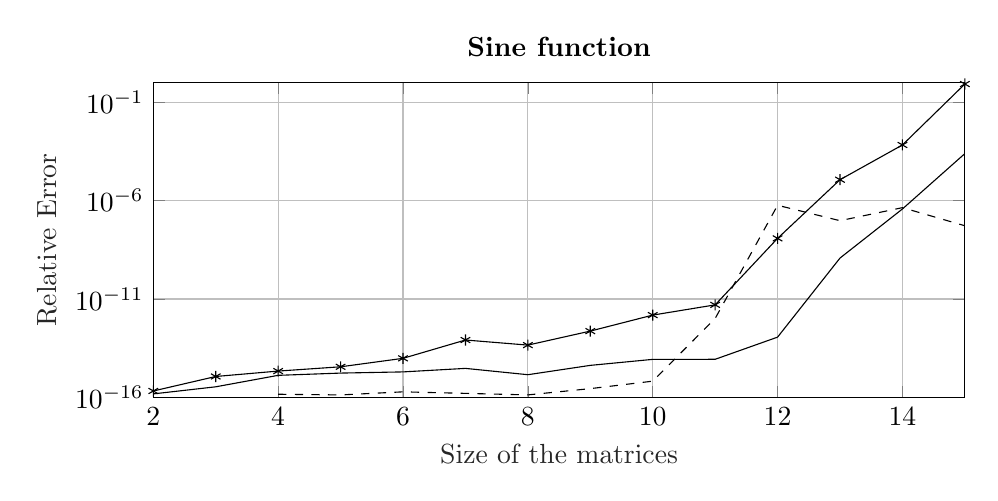
\begin{tikzpicture}

\begin{axis}[%
width=.85\linewidth,
height=4cm,
at={(0in,0in)},
scale only axis,
xmin=2,
xmax=15,
xlabel style={font=\color{white!15!black}},
xlabel={Size of the matrices},
ymode=log,
ymin=1e-16,
ymax=1,
yminorticks=true,
ylabel style={font=\color{white!15!black}},
ylabel={Relative Error},
axis background/.style={fill=white},
title style={font=\bfseries},
title={Sine function},
xmajorgrids,
ymajorgrids,
yminorgrids,
legend style={legend cell align=left, align=left, draw=white!15!black}
]
\addplot [color=black, dashed]
  table[row sep=crcr]{%
1	0\\
2	0\\
3	0\\
4	1.45725786217287e-16\\
5	1.34599448599507e-16\\
6	1.93288933939941e-16\\
7	0\\
8	1.34996517212839e-16\\
9	2.8139452012619e-16\\
10	6.73147337595159e-16\\
11	1.03032779116962e-12\\
12	5.78744177027967e-07\\
13	9.553747250617e-08\\
14	4.39017470636033e-07\\
15	5.28442449627079e-08\\
};
%\addlegendentry{diagonal}

\addplot [color=black, mark=asterisk, mark options={solid, black}]
  table[row sep=crcr]{%
1	0\\
2	2.13550872140361e-16\\
3	1.16425372303465e-15\\
4	2.19221444950359e-15\\
5	3.61672445574946e-15\\
6	9.72750676886519e-15\\
7	8.29608424074529e-14\\
8	4.56885037269095e-14\\
9	2.35417884883477e-13\\
10	1.52796832107972e-12\\
11	5.06284131371555e-12\\
12	1.20831615925066e-08\\
13	1.15240427666526e-05\\
14	0.000671713459124643\\
15	0.837016575460994\\
};
%\addlegendentry{symmetric}

\addplot [color=black]
  table[row sep=crcr]{%
1	0\\
2	1.51944372493216e-16\\
3	3.48056882596735e-16\\
4	1.33057104500803e-15\\
5	1.73250362957786e-15\\
6	1.99001209845091e-15\\
7	3.0020193056546e-15\\
8	1.43307608835298e-15\\
9	4.27119186288929e-15\\
10	8.62089393846284e-15\\
11	8.69296395513068e-15\\
12	1.16168249112529e-13\\
13	1.20836095810293e-09\\
14	3.76245413376949e-07\\
15	0.000244683076230114\\
};
%\addlegendentry{dense}

\end{axis}
\end{tikzpicture}%
        \caption{}
        \label{fig:comp_sine}
    \end{subfigure}\hspace{.055\linewidth}
    \begin{subfigure}[b]{0.3\textwidth}
        % This file was created by matlab2tikz.
%
%The latest updates can be retrieved from
%  http://www.mathworks.com/matlabcentral/fileexchange/22022-matlab2tikz-matlab2tikz
%where you can also make suggestions and rate matlab2tikz.
%
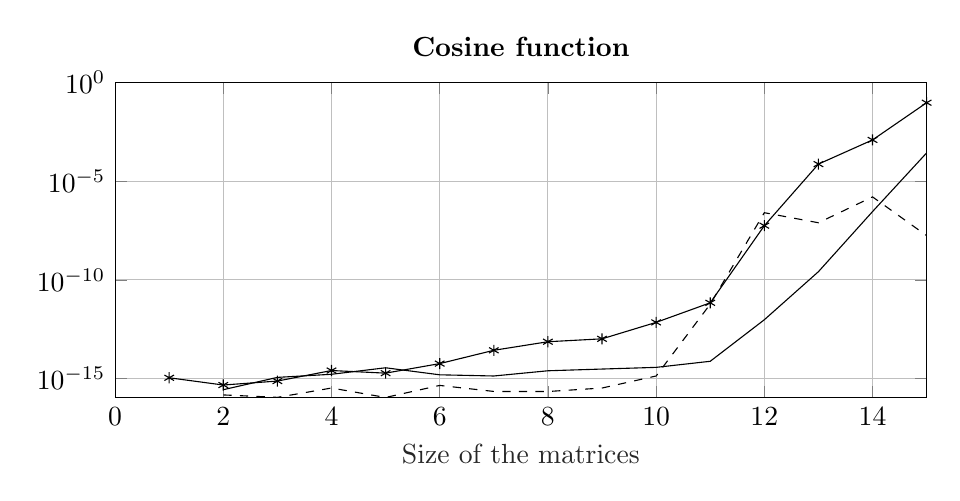
\begin{tikzpicture}

\begin{axis}[%
width=.85\linewidth,
height=4cm,
at={(0in,0in)},
scale only axis,
xmin=0,
xmax=15,
xlabel style={font=\color{white!15!black}},
xlabel={Size of the matrices},
ymode=log,
ymin=1.1104582787894e-16,
ymax=1,
yminorticks=true,
ylabel style={font=\color{white!15!black}},
%ylabel={Relative Error},
axis background/.style={fill=white},
title style={font=\bfseries},
title={Cosine function},
xmajorgrids,
ymajorgrids,
yminorgrids,
legend style={legend cell align=left, align=left, draw=white!15!black}
]
\addplot [color=black, dashed]
  table[row sep=crcr]{%
1	0\\
2	1.49254976159848e-16\\
3	1.12386960222902e-16\\
4	3.33629533162353e-16\\
5	1.1104582787894e-16\\
6	4.51664304824148e-16\\
7	2.24222591598726e-16\\
8	2.22284366724468e-16\\
9	3.3326394200314e-16\\
10	1.35535886136552e-15\\
11	5.90120769250069e-12\\
12	2.53895186073711e-07\\
13	7.86074239881932e-08\\
14	1.60599491859353e-06\\
15	1.74974849891932e-08\\
};
%\addlegendentry{diagonal}

\addplot [color=black, mark=asterisk, mark options={solid, black}]
  table[row sep=crcr]{%
1	1.10216884990089e-15\\
2	4.73392519955033e-16\\
3	7.52201284293378e-16\\
4	2.56983598583253e-15\\
5	1.8934958043445e-15\\
6	5.76079452953616e-15\\
7	2.71936809409104e-14\\
8	7.38660809880766e-14\\
9	1.03575975843225e-13\\
10	7.05810087502504e-13\\
11	6.91539504160167e-12\\
12	5.58866941125034e-08\\
13	7.35834262695204e-05\\
14	0.00123336328753215\\
15	0.0944453153509049\\
};
%\addlegendentry{symmetric}

\addplot [color=black]
  table[row sep=crcr]{%
1	0\\
2	2.74801956341246e-16\\
3	1.15411270860285e-15\\
4	1.65853388726515e-15\\
5	3.54103245149018e-15\\
6	1.5589802910102e-15\\
7	1.35811075119445e-15\\
8	2.49648348011263e-15\\
9	3.05245869225958e-15\\
10	3.71275847951212e-15\\
11	7.54587960659731e-15\\
12	9.59882062625648e-13\\
13	2.61418513595533e-10\\
14	2.89445409507326e-07\\
15	0.000271321657431055\\
};
%\addlegendentry{dense}

\end{axis}
\end{tikzpicture}%
        \caption{}
        \label{fig:comp_cosine}
    \end{subfigure}\hspace{.025\linewidth}
    \begin{subfigure}[b]{0.3\textwidth}
        % This file was created by matlab2tikz.
%
%The latest updates can be retrieved from
%  http://www.mathworks.com/matlabcentral/fileexchange/22022-matlab2tikz-matlab2tikz
%where you can also make suggestions and rate matlab2tikz.
%
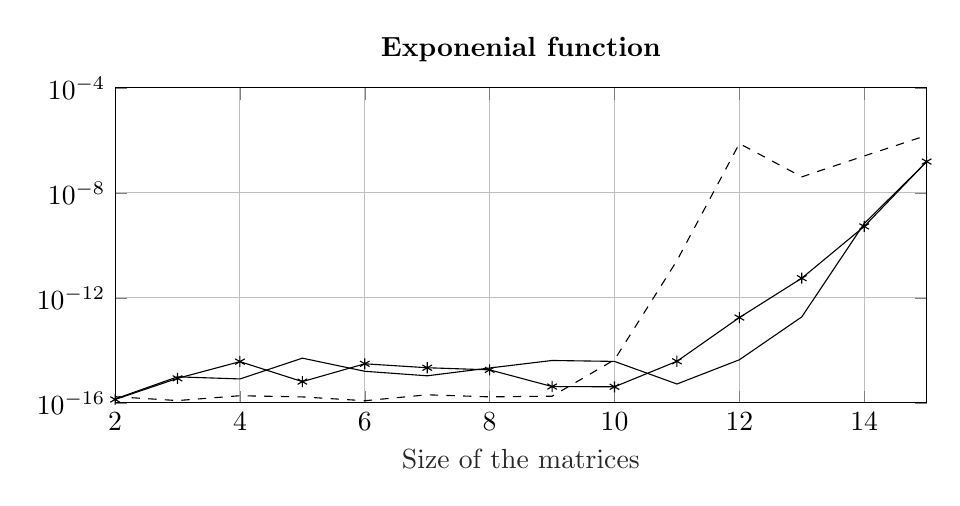
\begin{tikzpicture}

\begin{axis}[%
width=.85\linewidth,
height=4cm,
at={(0in,0in)},
scale only axis,
xmin=2,
xmax=15,
xlabel style={font=\color{white!15!black}},
xlabel={Size of the matrices},
ymode=log,
ymin=1e-16,
ymax=0.0001,
yminorticks=true,
ylabel style={font=\color{white!15!black}},
%ylabel={Relative Error},
axis background/.style={fill=white},
title style={font=\bfseries},
title={Exponenial function},
xmajorgrids,
ymajorgrids,
yminorgrids,
legend style={legend cell align=left, align=left, draw=white!15!black}
]
\addplot [color=black, dashed]
  table[row sep=crcr]{%
1	0\\
2	1.71624878976539e-16\\
3	1.22024250623032e-16\\
4	1.86764659618892e-16\\
5	1.68361863632822e-16\\
6	1.20424787755581e-16\\
7	2.02522198739353e-16\\
8	1.69083627914502e-16\\
9	1.78878188543304e-16\\
10	4.37883232600663e-15\\
11	2.62205407924652e-11\\
12	7.55548252824038e-07\\
13	4.08147804640456e-08\\
14	2.54902728221652e-07\\
15	1.54338995955608e-06\\
};
%\addlegendentry{diagonal}

\addplot [color=black, mark=asterisk, mark options={solid, black}]
  table[row sep=crcr]{%
1	0\\
2	1.34551194988101e-16\\
3	8.56940672084931e-16\\
4	3.71431920865263e-15\\
5	6.43853140792487e-16\\
6	3.07364008605186e-15\\
7	2.17447874006037e-15\\
8	1.80680598636716e-15\\
9	4.18315732440152e-16\\
10	4.08961300873358e-16\\
11	3.83448312676478e-15\\
12	1.77593347794744e-13\\
13	5.61443457608614e-12\\
14	5.25277002444549e-10\\
15	1.55722814732103e-07\\
};
%\addlegendentry{symmetric}

\addplot [color=black]
  table[row sep=crcr]{%
1	0\\
2	1.40422527187022e-16\\
3	9.78212455490046e-16\\
4	8.14581110397033e-16\\
5	5.04209119228841e-15\\
6	1.59210015961528e-15\\
7	1.07228002023245e-15\\
8	2.12873989764519e-15\\
9	4.11404419473943e-15\\
10	3.79263905604626e-15\\
11	5.22236059957374e-16\\
12	4.37354475237039e-15\\
13	1.88271014260457e-13\\
14	6.79585192457534e-10\\
15	1.52106181005324e-07\\
};
%\addlegendentry{dense}

\end{axis}
\end{tikzpicture}%
        \caption{}
        \label{fig:comp_exp}
    \end{subfigure}
    \caption{Measure of performance of the algorithm to compute $f(\mathbf{A})$ according to definition \ref{def:Hermite}. We assume that \cite{davies2003schur} (Schur Parlett) algorithm is correct, and we measure the relative error. We compare the performance of our algorithm on several types of matrices : diagonal (- -), symmetric (-*) and dense (--). Matrix coefficients are randomly filled such that for all non-zero entry: $a_{ij}\sim\mathcal{U}(0,1)$, this ensures $\mathbf{A}$ is full rank. We test it on three different functions : Sine (a), Cosine (b) and Exponenial (c). We note that starting from a certain matrix size, the algorithm lose considerably in performance.}
    \label{fig:comp}
\end{figure}

Figure \ref{fig:comp} illustrate the result of the measurement of performance of the algorithm. The relative error between \cite{davies2003schur} and our results is computed:
\begin{equation*}
    \text{relative error} = \frac{\|f(\mathbf{A})-\texttt{funm}(\mathbf{A},f)\|_2}{\|\texttt{funm}(\mathbf{A},f\|_2}
\end{equation*}
\section{Applications}
\subsection{Matrix Exponential}\label{sec:matrixexp}
Consider the simple system of ODEs
\begin{equation}\label{eq:ode}
    \frac{d\mathbf{x}}{dt} = \mathbf{A}\mathbf{x}
\end{equation}
with initial condition $\mathbf{x}(0) = \mathbf{x}_0\in\mathbb{R}^n$. Then we know the solution to be given by $\mathbf{x}(t)=e^{\mathbf{A}t}\mathbf{x}_0$. However, for all but the stablest systems, this is not a good method, due to issues such as stability and stiffness. Here we consider for instance the 2D convection-diffusion equation for the flow $\mathbf{u}(x,y)$:
$$\frac{d \mathbf{u}}{d t}=\epsilon\Delta\mathbf{u}+\alpha\cdot\nabla\mathbf{u}$$
with Dirichlet boundary conditions and $\epsilon\in\mathbb{R}^{+}_0$ and $\alpha\in\mathbb{R}^2$. Simple time-stepping methods are known to be unstable at large time-steps, and our exponential scheme suffers from similar problems, i.e. $t$ cannot be taken too large.
\subsection{The sign function}
In control theory we are often interested in the eigenvalues $\lambda$ of system matrices with $Re(\lambda)>0$, since they correspond to unstable poles. In the design of controllers it is therefore interesting to have an efficient way to count the number of eigenvalues of a matrix in the right half-plane $Re(z)>0$. Here we will build such a method.
\begin{theorem}\label{thm:sign}
Let $\mathbf{A}\in\mathbb{C}^{n \times n}$ be a matrix with $k_{-}$ eigenvalues in the left plane, $k_{+}$ eigenvalues in the right plane and none on the imaginary axis, counting multiplicity. Let $\text{sgn}:\mathbb{C}\mapsto \{1,-1\}$ be defined by
$$\text{sgn}(z)= \begin{cases} 
      1 & Re(z)\geq 0 \\
      -1 & Re(z)<0. 
   \end{cases}
$$
Then $\text{trace}(\text{sgn}(\mathbf{A}))=k_{+}-k_{-}$.
\end{theorem}
\begin{proof}
    Let $\mathbf{A}\in\mathbb{C}^{n\times n}$. To stay in a very general scenario, and consider cases where $\mathbf{A}$, let us consider its Jordan Canonical Form :
    \begin{equation*}
        \mathbf{A} = \mathbf{VJV}^{-1}
    \end{equation*} 
    Recall that by theorem \ref{thm:jordan}, consider $f$ a function, then 
    \begin{equation*}
        f(\mathbf{A}) = \mathbf{V}f(\mathbf{J})\mathbf{V}^{-1}
    \end{equation*}
    Thus let us consider the decomposition where 
    \begin{equation*}
        \mathbf{J} = \begin{pmatrix}
            \mathbf{J}_{k_+} & 0 \\ 0 & \mathbf{J}_{k_-}
        \end{pmatrix}
    \end{equation*}
    such that $\mathbf{J}_{k_+}$ has $k_+$ eigenvalues in the right plane, and $\mathbf{J}_{k_-}$ has $k_-$ eigenvalues in the left plane. Then, we have that
    \begin{equation*}
        \text{sgn}(\mathbf{J}) = \begin{pmatrix}
            \mathbf{I}_{k_+} & 0 \\ 0 & -\mathbf{I}_{k_-}
        \end{pmatrix}
    \end{equation*}
    where $\mathbf{I}_n$ is the identity matrix of size $n$. Then, we have that
    \begin{equation*}
        \text{trace}(\text{sgn}(\mathbf{J})) = k_+ - k_-
    \end{equation*}
    And thus, we have that
    \begin{equation*}
        \text{trace}(\text{sgn}(\mathbf{A})) = \text{trace}(\text{sgn}(\mathbf{VJV}^{-1})) = \mathbf{V}\text{trace}(\text{sgn}(\mathbf{J}))\mathbf{V}^{-1} = (k_+-k_-)\mathbf{V}\mathbf{V}^{-1} = k_+ - k_-
    \end{equation*}
\end{proof}
\printbibliography
\end{document}